\documentclass{beamer}

\mode<presentation> {

\usetheme{CambridgeUS} %%
%\usetheme{Darmstadt} %%
%\usetheme{Madrid}

% To remove the footer line in all slides uncomment this line
%\setbeamertemplate{footline}

% To replace the footer line in all slides with a simple slide count uncomment this line
%\setbeamertemplate{footline}[page number]

% To remove the navigation symbols from the bottom of all slides uncomment this line
%\setbeamertemplate{navigation symbols}{}
}

\usepackage{graphicx} % Allows including images
\usepackage{booktabs} % Allows the use of \toprule, \midrule and \bottomrule in tables
\usepackage{multimedia} % Insertion video
\usepackage{wrapfig}

%----------------------------------------------------------------------------------------
%	TITLE PAGE
%----------------------------------------------------------------------------------------

\title[Projet Micro\'electronique 2A SEI]{Projet de Conception en Micro\'electronique Analogique \\ R\'ealisation d'un CAN FLASH 6 bits }
% The short title appears at the bottom of every slide, the full title is only on the title page
%\subtitle{Test}

\author{F. Goumis, M. Hage Hassan} % Your name
\institute[Phelma] % Your institution as it will appear on the bottom of every slide, may be shorthand to save space
{
Institut Polytechnique de Grenoble - Phelma\\ % Your institution for the title page
\medskip
\textit{mohamed.hage-hassan@phelma.grenoble-inp.fr}\\ % Your email address
\textit{ferdinand.goumis@phelma.grenoble-inp.fr}
}

\date{\today} % Date, can be changed to a custom date

\begin{document}

\begin{frame}
\titlepage % Print the title page as the first slide
\end{frame}

%----------------------------------------------------------------------------------------
%	PRESENTATION SLIDES
%----------------------------------------------------------------------------------------

\begin{frame}
\frametitle{D\'emarches}

\tableofcontents

\end{frame}

\section{Cahier des charges} % A subsection can be created just before a set of slides with a common theme
%to further break down your presentation into chunks

%------------------------------------------------

\begin{frame}
\frametitle{Cahier des charges}

\begin{columns}[T]
  \column{0.5\textwidth}
  \begin{itemize}
    \item[-] Une r\'esolution du CAN-FLASH de 6 bits\\ce qui implique l'utilisation de $2^{6} -1 = 63 $ comparateurs.
    \item[-] Dynamique du signal en entr\'ee $V_e \in [0.5 V,\phantom{2} 2.5V]$
    \item[-] Fr\'equence d'\'echantillonnage : $f_h = 20 MHz $
  \end{itemize}

  \column{0.4\textwidth}
  \hspace*{-0.5cm}
  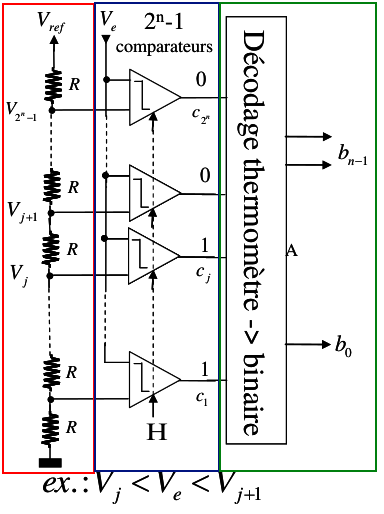
\includegraphics[width=0.9\linewidth]{schema_global_charges.png}
\end{columns}

\end{frame}

%------------------------------------------------

\section{Mise en place de l'\'echantillonneur-bloqueur}

\begin{frame}
\frametitle{Principe de Fonctionnement}

\begin{figure}[!htb]
\begin{center}
  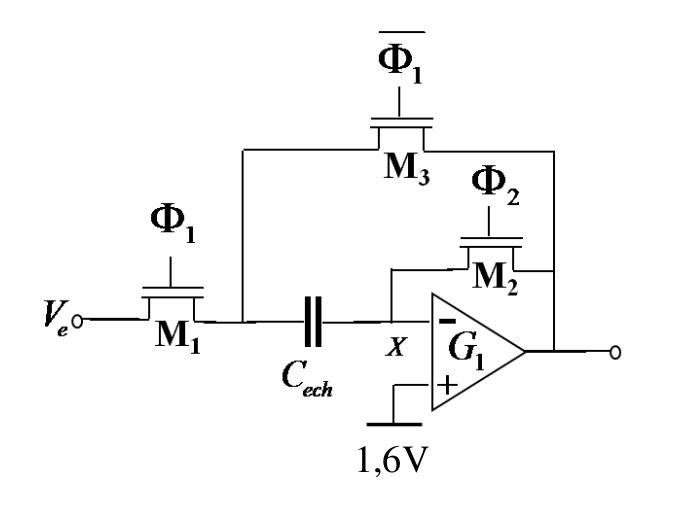
\includegraphics[width=0.4\linewidth]{Echantillonneur-bloqueur.jpg}
  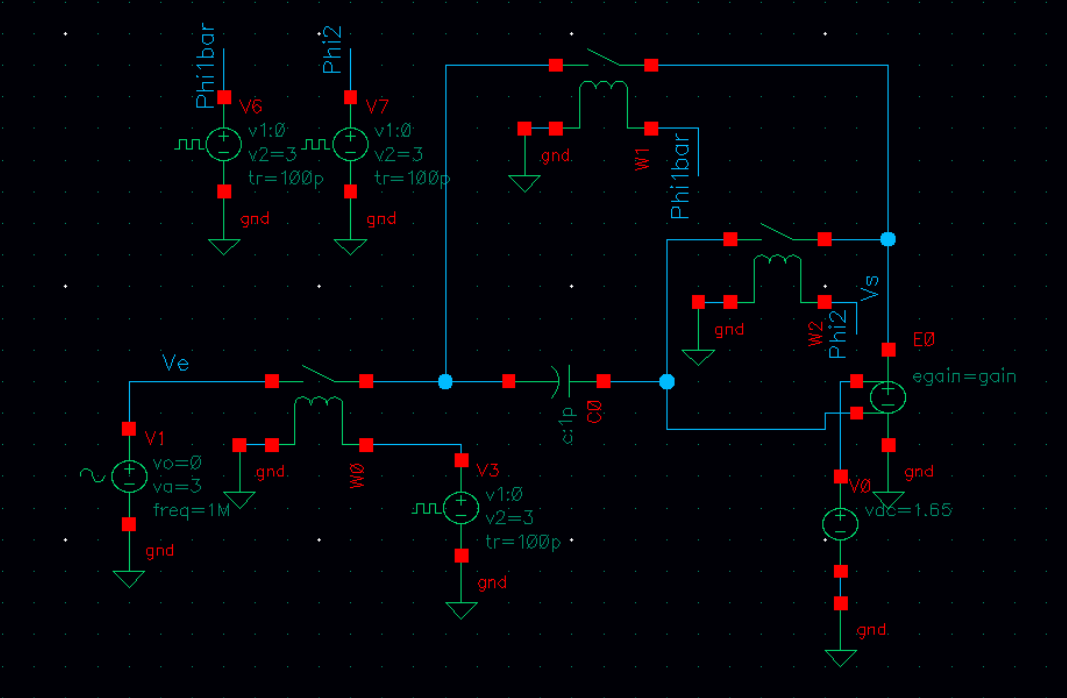
\includegraphics[width=0.6\linewidth]{Echantillonneur-bloqueur_ideal.png}
  \caption{Sch\'ema \'electrique de l'\'echantillonneur-bloqueur}
\end{center}
\end{figure}

\end{frame}

%------------------------------------------------

\begin{frame}
\frametitle{Simulation id\'eale}

\begin{figure}[!htb]
\begin{center}
  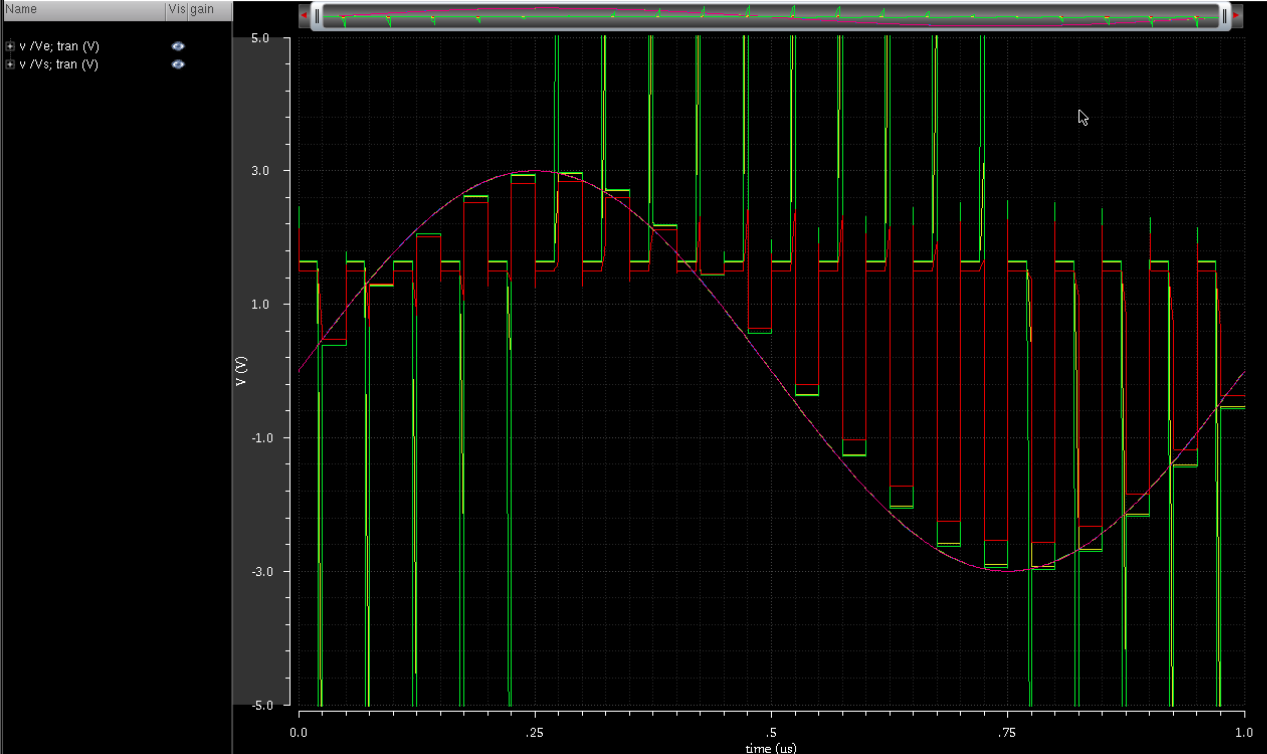
\includegraphics[width=0.7\linewidth]{simu_ech_bloqueur_ideal.png}
  \caption{Simulation de l'\'echantillonneur-bloqueur \`a \'elements id\'eaux}
\end{center}
\end{figure}

\end{frame}

%------------------------------------------------

\begin{frame}
\frametitle{R\'ealisation des switchs}

\textbf{Addition des trucs}

\begin{columns}[T]
  \column{0.4\textwidth}
  \begin{itemize}
    \item[-] Une r\'esolution du CAN-FLASH de 6 bits\\ce qui implique l'utilisation de $2^{6} -1 = 63 $ comparateurs.
  \end{itemize}
  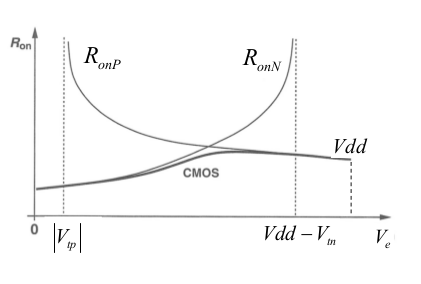
\includegraphics[width=0.9\linewidth]{switch_fonct.png}

  \column{0.6\textwidth}
  \hspace*{-0.5cm}
  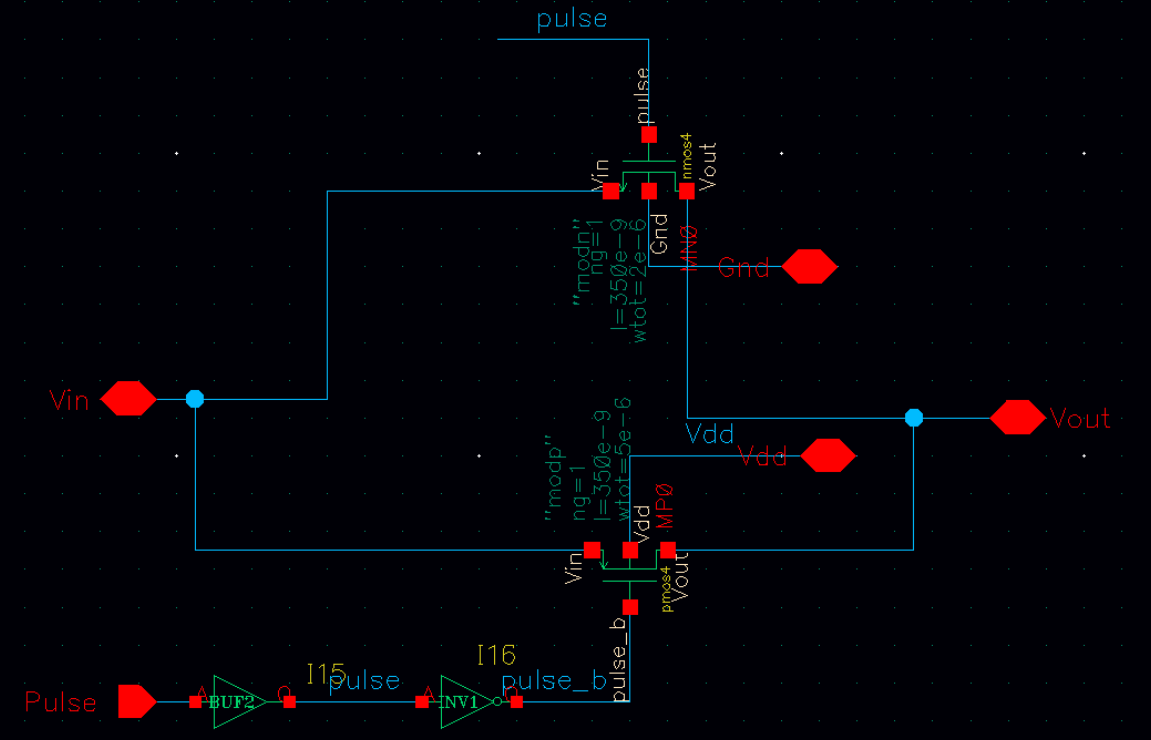
\includegraphics[width=\linewidth]{switchs_.png}
\end{columns}

\end{frame}

%------------------------------------------------

\begin{frame}
\frametitle{Simuation des switchs}

\begin{figure}[!htb]
  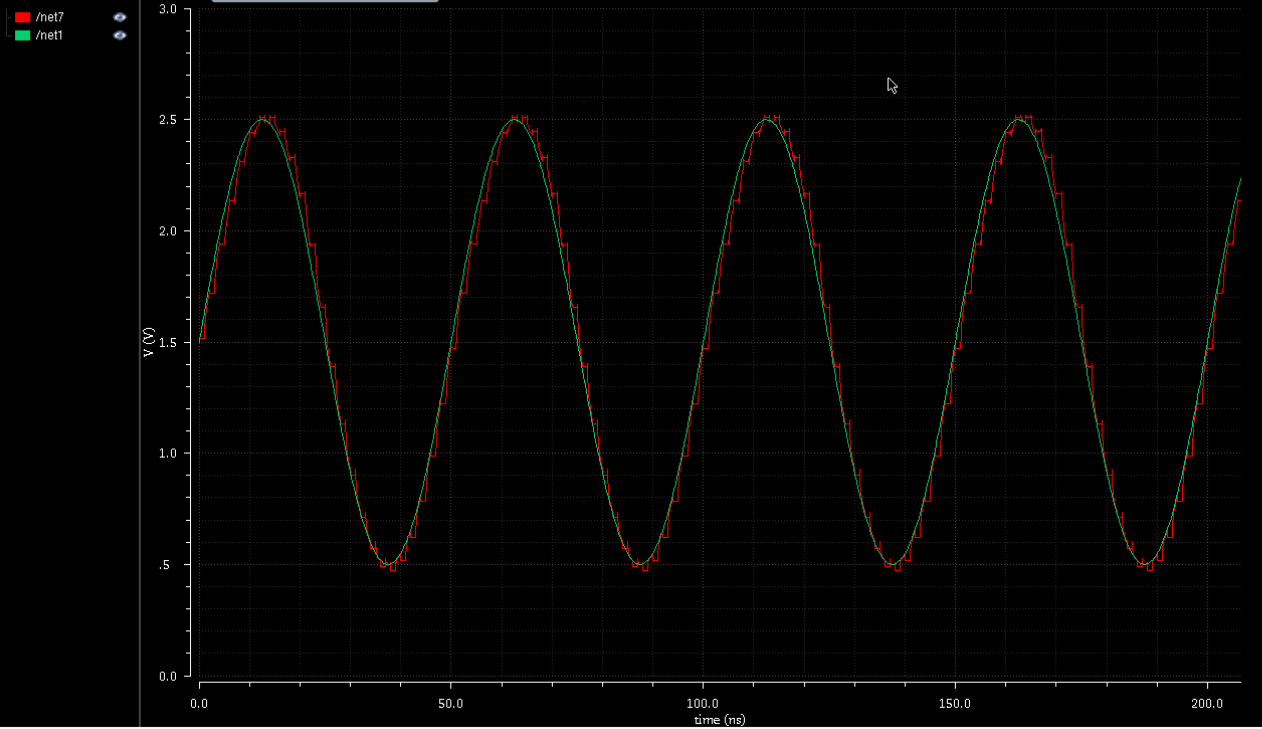
\includegraphics[width=0.7\linewidth]{switchs_simu.png}
  \caption{Simulation des switchs en CMOS}
\end{figure}

\end{frame}

%------------------------------------------------

\begin{frame}
\frametitle{Sch\'ema r\'eel}

\begin{figure}[!htb]
  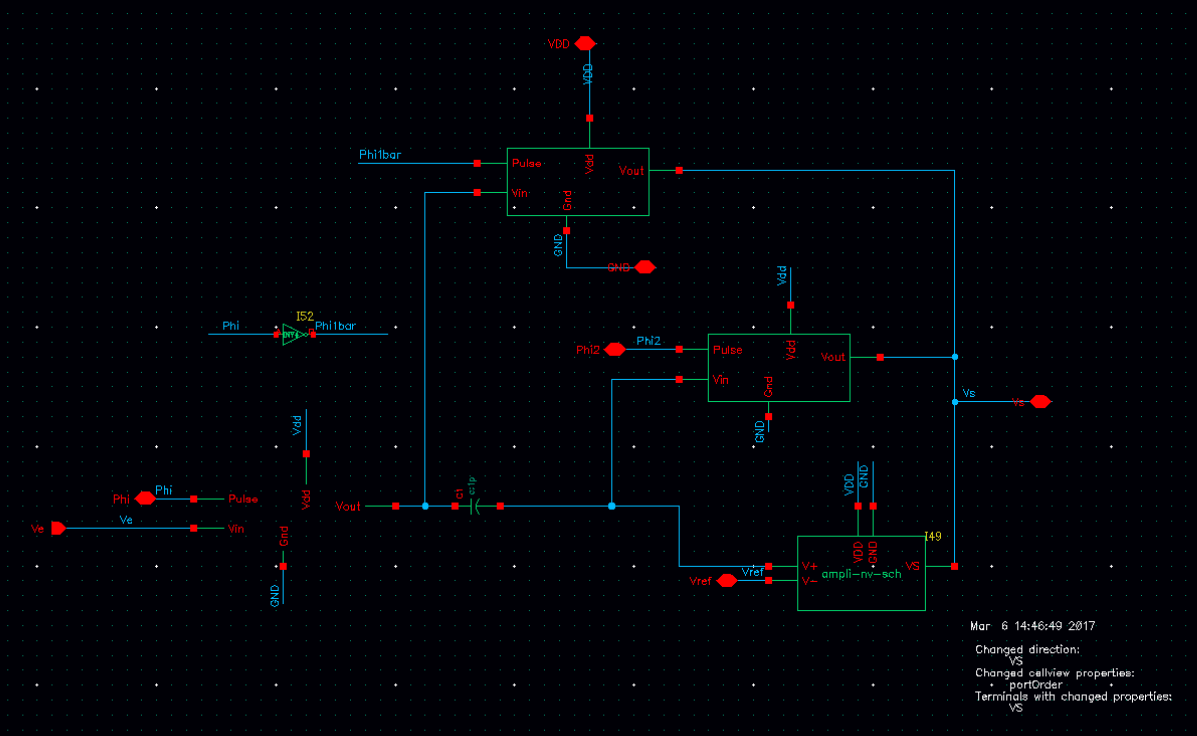
\includegraphics[width=0.7\linewidth]{EB-Schematic.png}
  \caption{Simulation des switchs en CMOS}
\end{figure}

\end{frame}

%------------------------------------------------


\section{R\'ealisation d'un Amplificateur OTA \`a deux \'etages}

\begin{frame}
\frametitle{Fonctionnement}

\begin{figure}[!htb]
  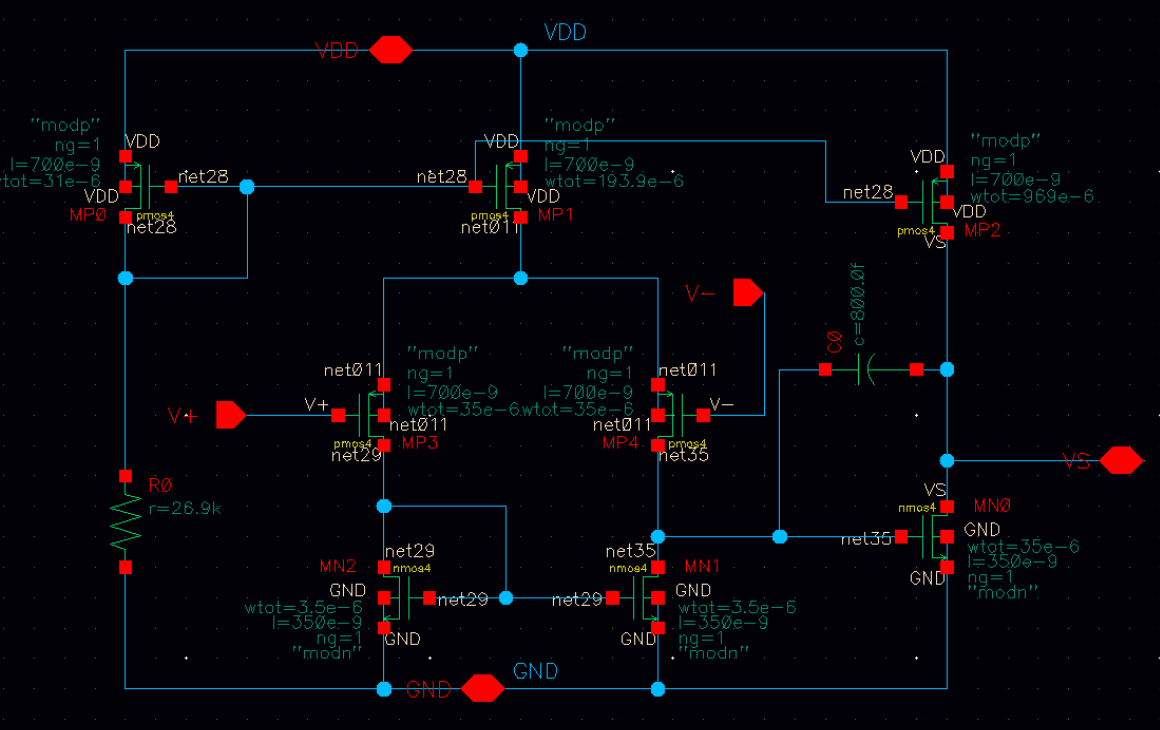
\includegraphics[width=0.7\linewidth]{amplificateur_.png}
  \caption{Simulation des switchs en CMOS}
\end{figure}

\end{frame}

%------------------------------------------------

\begin{frame}
\frametitle{Simulation de l'amplificateur \`a deux \'etages}

\begin{figure}[!htb]
  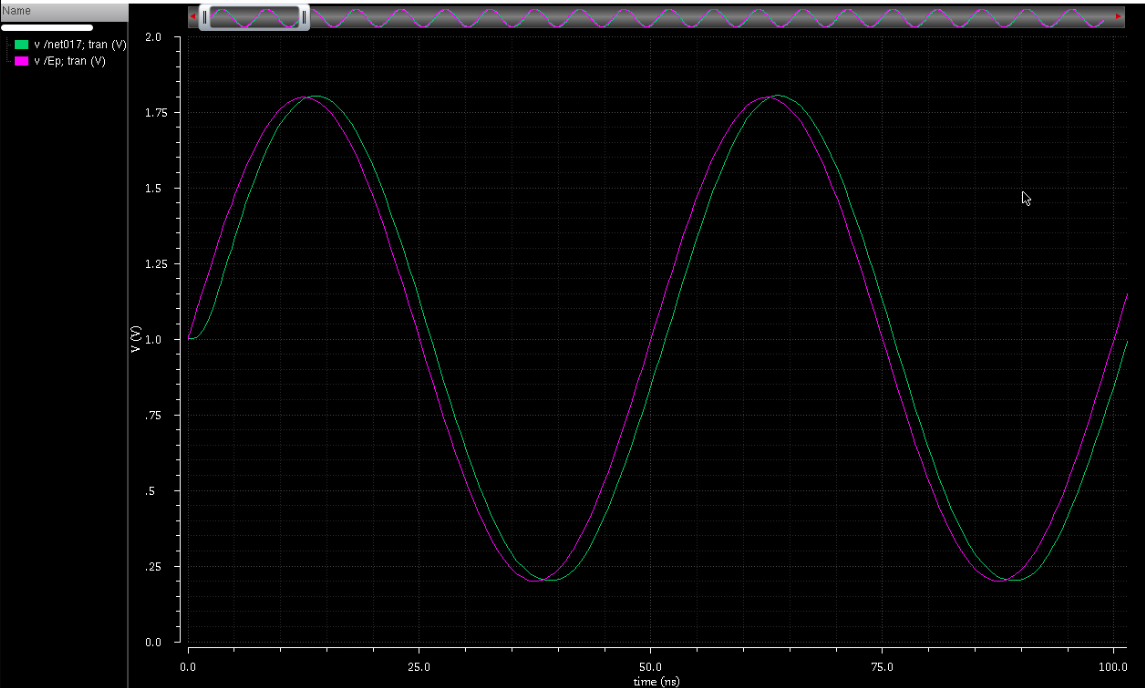
\includegraphics[width=0.8\linewidth]{reponse_ampli.png}
  \caption{Simulation de l'amplificateur}
\end{figure}

\end{frame}

\begin{frame}
\frametitle{Simulation de l'amplificateur \`a deux \'etages - Analyse fr\'equentielle}

\begin{figure}[!htb]
  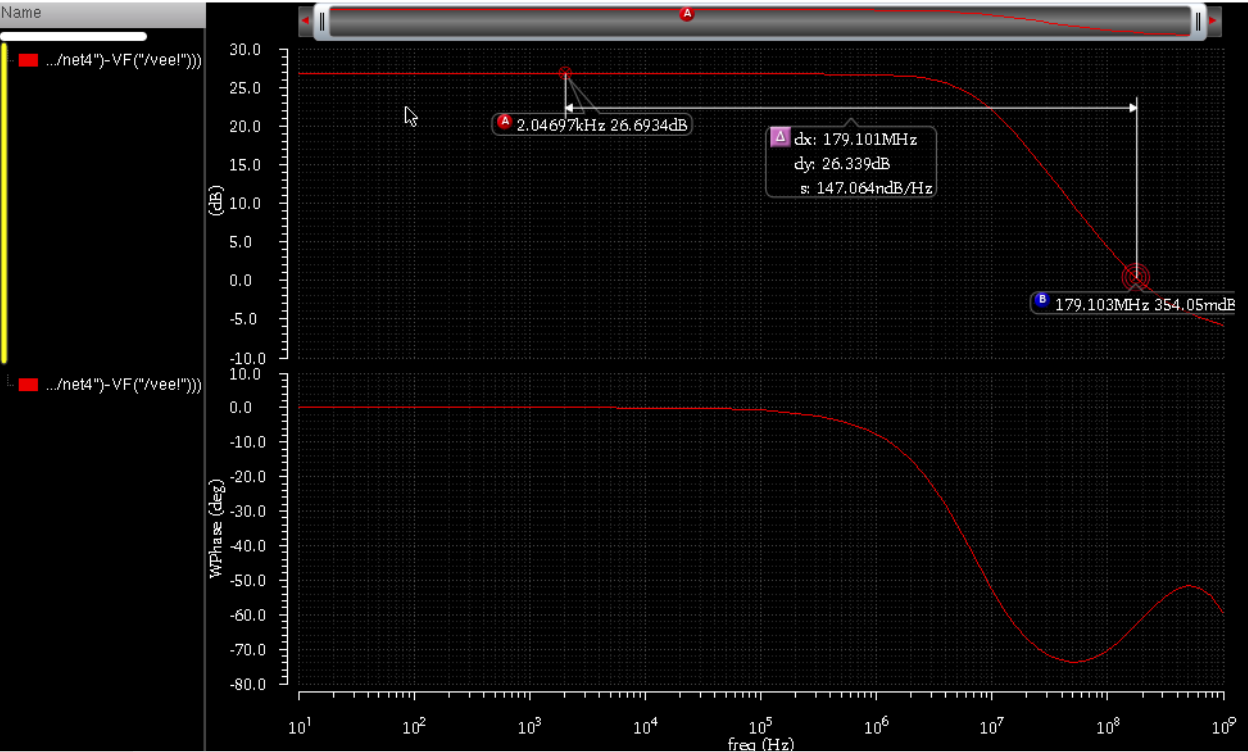
\includegraphics[width=0.8\linewidth]{ampli_bode.png}
  \caption{Simulation de l'amplificateur en AC}
\end{figure}

\end{frame}

%------------------------------------------------

\begin{frame}
\frametitle{Simulation final de l'Echantillonneur bloqueur}

\begin{figure}[!htb]
  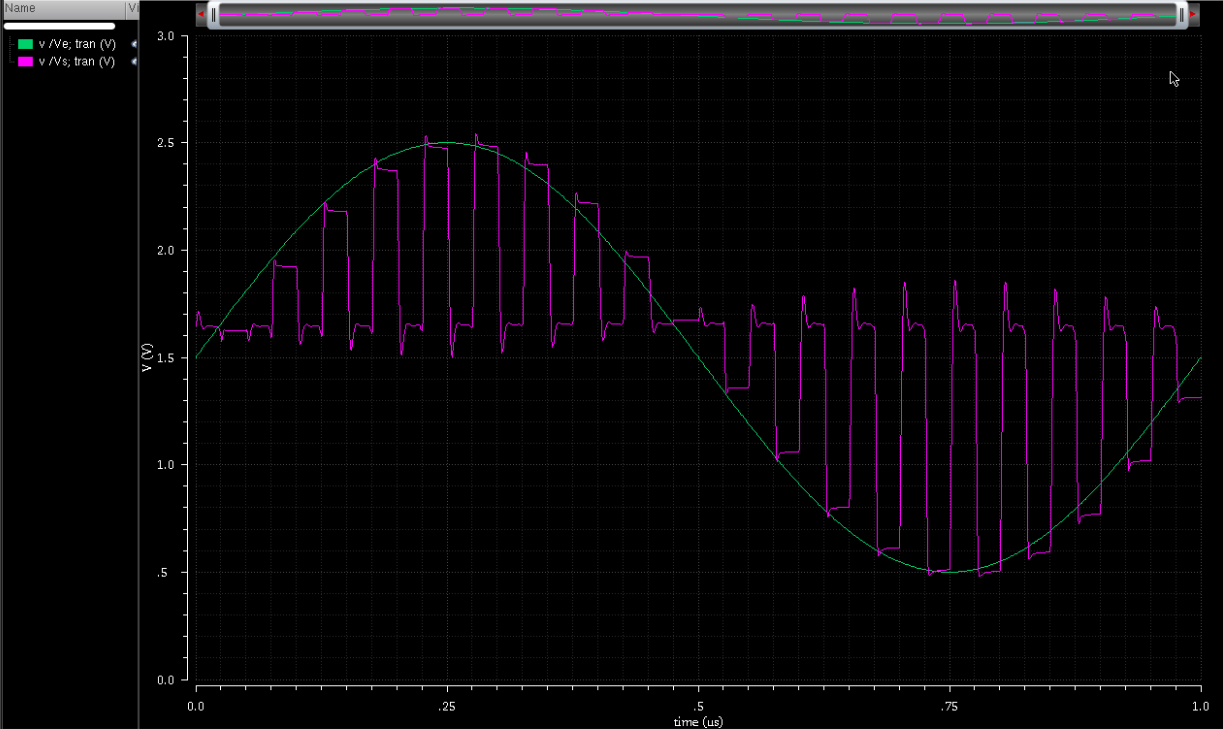
\includegraphics[width=0.8\linewidth]{echantillonneur_bloqueur_sim_reelle.png}
  \caption{Simulation finale}
\end{figure}

\end{frame}


\section{Mise en oeuvre des comparateurs synchronis\'es par horloge}

\begin{frame}
\frametitle{Fonctionnement}

\begin{figure}[!htb]
  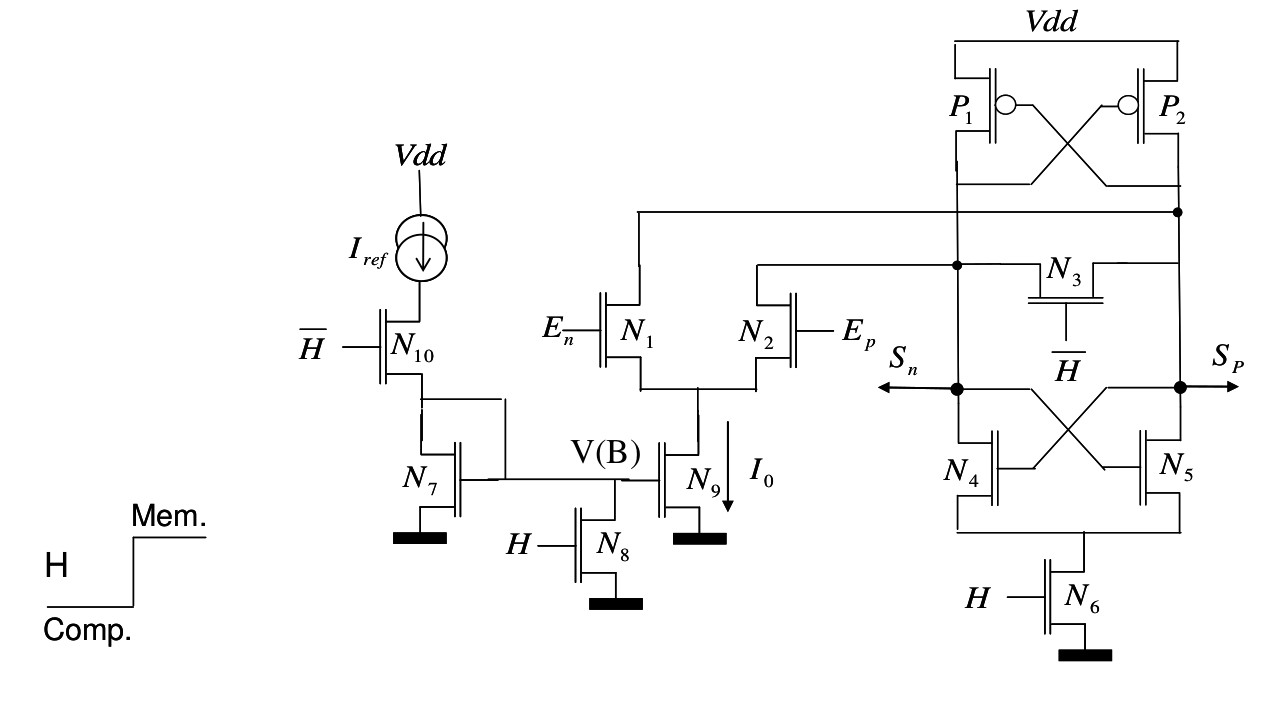
\includegraphics[width=0.8\linewidth]{comparateur_schema.jpg}
  \caption{Simulation finale}
\end{figure}

\end{frame}

%------------------------------------------------

\begin{frame}
\frametitle{Simulation}

\begin{figure}[!htb]
  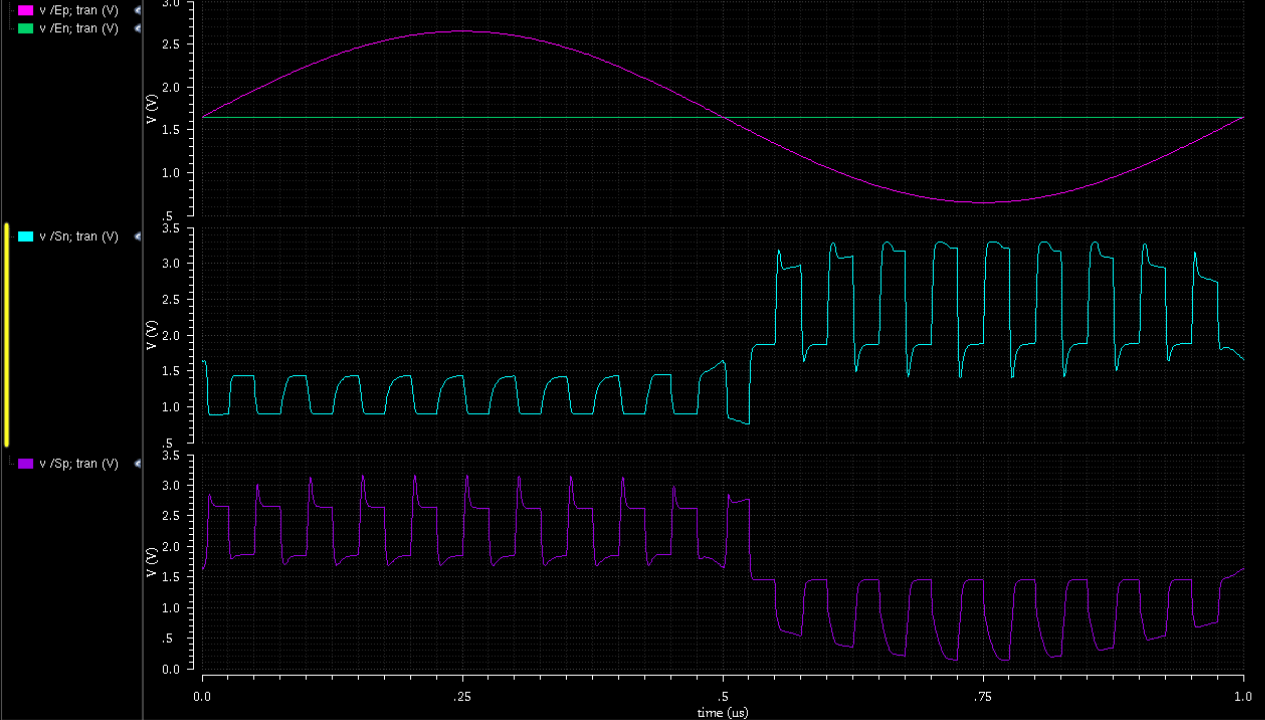
\includegraphics[width=0.8\linewidth]{simu_comp_pas_ameliore.png}
  \caption{Simulation finale}
\end{figure}

\end{frame}

%------------------------------------------------

\begin{frame}
\frametitle{Modification n\'ecessaires}

\begin{figure}[!htb]
  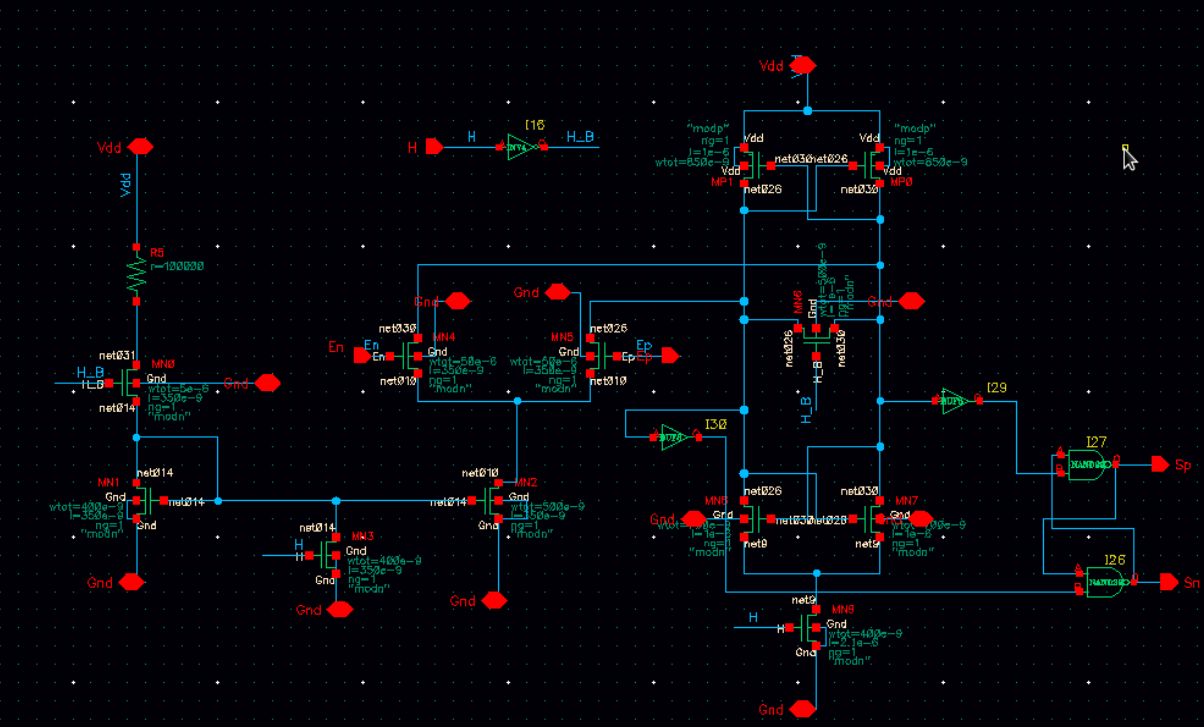
\includegraphics[width=0.8\linewidth]{comparateur_schema_cadence_SR.png}
  \caption{Addition des buffers et Bascules SR}
\end{figure}

\end{frame}

%------------------------------------------------

\begin{frame}
\frametitle{Simulation apr\`es modifications}

\begin{figure}[!htb]
  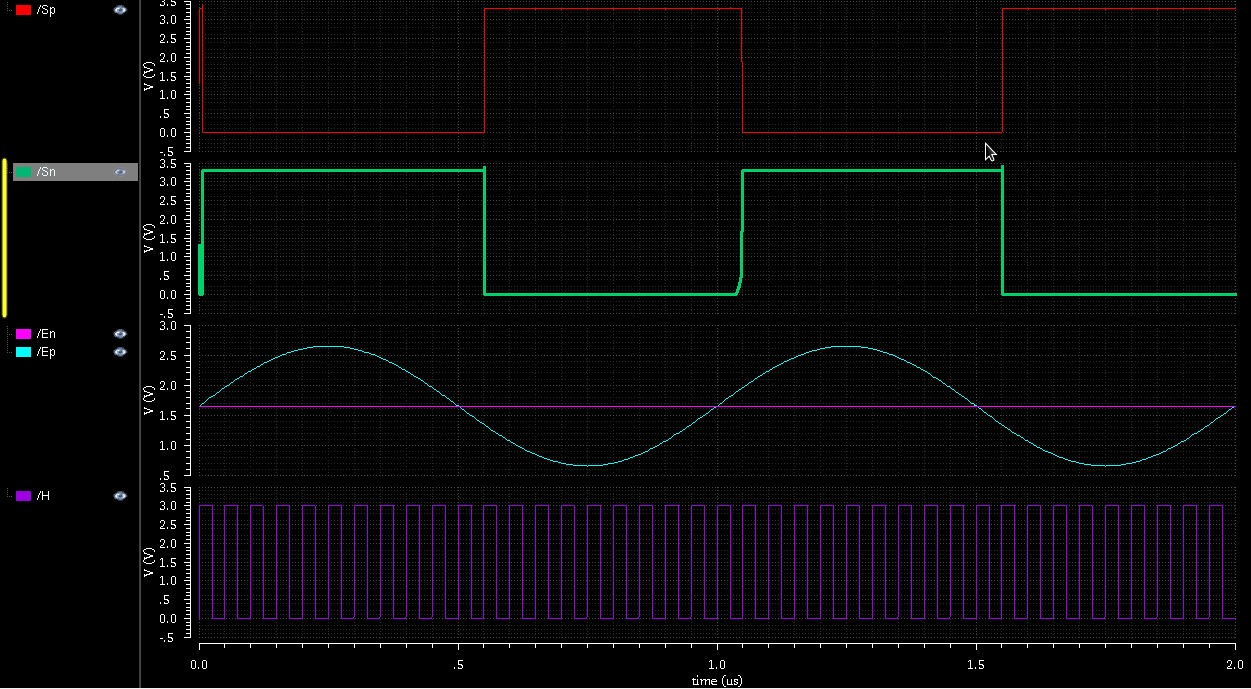
\includegraphics[width=0.8\linewidth]{sim_comp_after_SR_FF.jpg}
  \caption{Addition des buffers et Bascules SR}
\end{figure}

\end{frame}


\section{R\'ealisation du d\'ecodeur en Verilog}

\begin{frame}
\frametitle{Synth\`ese}

\begin{figure}[!htb]
  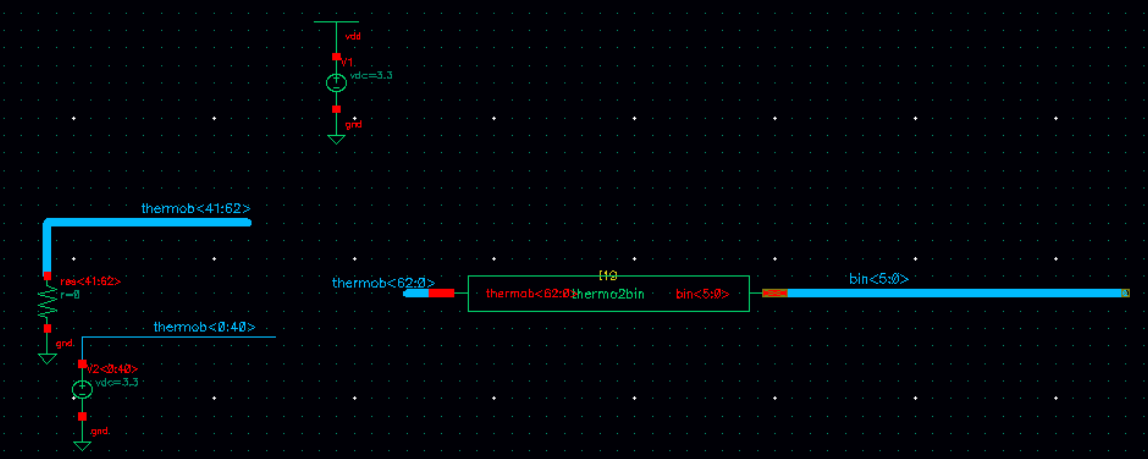
\includegraphics[width=0.8\linewidth]{test_thermo2bin.png}
  \caption{Test du codeur thermometrique}
\end{figure}

\end{frame}

%------------------------------------------------

\section{Sch\'ema Global}

\begin{frame}
\frametitle{Sch\'ema final}

\begin{figure}[!htb]
  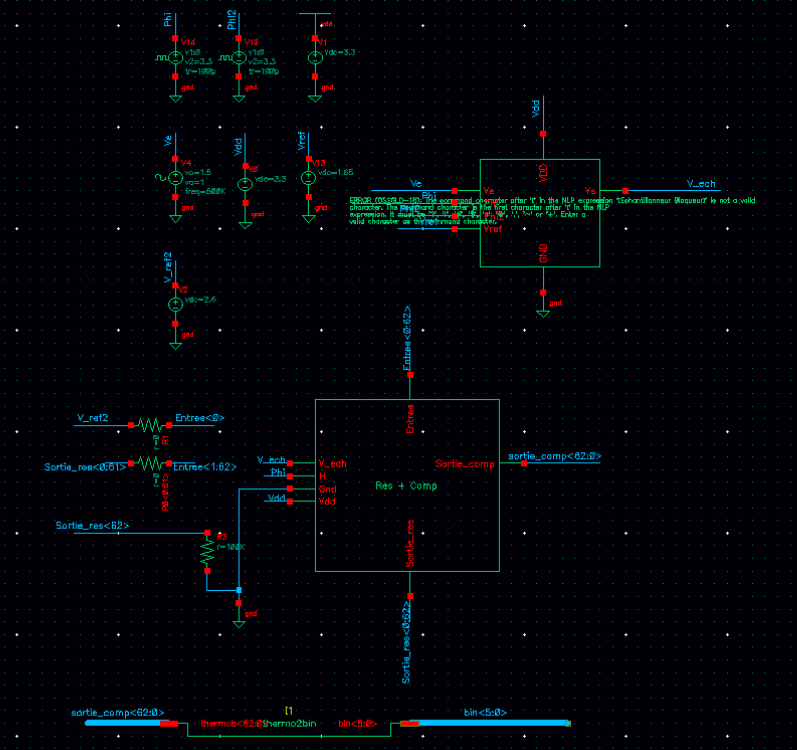
\includegraphics[width=0.6\linewidth]{schema_final.png}
  \caption{Test du codeur thermometrique}
\end{figure}

\end{frame}

%------------------------------------------------

\section{Layout}

\begin{frame}

\begin{figure}[!htb]
  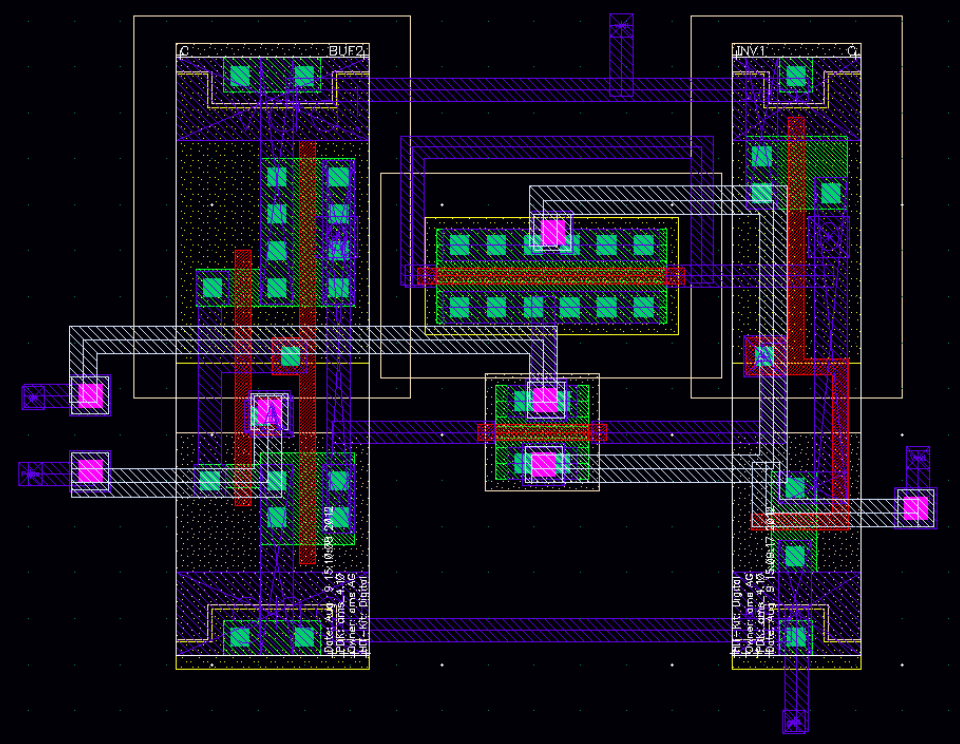
\includegraphics[width=0.6\linewidth]{layout_.png}
  \caption{Layout du switch}
\end{figure}

\end{frame}

%------------------------------------------------

\section{Conclusion/Am\'eliorations possibles}

\begin{frame}

\begin{itemize}
    \item Bon fonctionnement du CAN (3 erreurs sur 63 valeurs).
    \item R\'ealis\'e avec des \'el\'ements de base.
\end{itemize}

\medskip

\textbf{Am\'eliorations possibles}
\begin{itemize}
  \item Am\'elioration la polarisation de sortie du comparateur.
  \item Meilleure isolation entre le pont de r\'esistances et comporateurs.
  \item Int\'er\^et \`a la surface utilis\'ee et la consommation.
  \item Utilisation potentielle de transistors pour recr\'eer les seuils.
\end{itemize}


\end{frame}

%------------------------------------------------

\iffalse
\section{Annexes}

\begin{frame}
\frametitle{Annexes}


\end{frame}

\fi


\end{document}
